\section{Interessentanalyse}
Gruppen vil i dette afsnit undersøge diverse personer/grupper, der kan fungere som interessenter i projektet, altså en person der vil have nytte af eller kan bidrage til projektet. Herefter vil gruppen prioritere disse interessenter, alt efter hvor relevante de er i forhold til projektet.  

\textbf{O-løbere} \newline
For at den enkelte o-løber skal kunne forbedre, sig er det vigtig at kunne sammenligne løberens rute detaljeret med andre, lige nu er tiderne mellem hver post (stræktiderne) det eneste der kan sammenlignes og analyseres på. Her er det interessant for løberen at kigge på vejvalg og hastighed mellem posterne, og endda helt ned til de forskellige faser af delstrækkene. Til dette mangler der mere detaljeret data om løbet. Problemet håndteres i dag ved at sammenligne skemaer med stræktider og hvis muligt manuelt indtegne vejvalg på kortet efter løberens hukommelse. Derfor har den enkelte o-løber interesse i dette projekt da der arbejdes med afvikling og opfølgning af træningen. 

\textbf{Træneren}\newline
Træneren har interesse i at gøre de enkelte løbere bedre, træneren har derfor også interesse i at mindske arbejet på planlægning og forberedelse af træningen, da der bruges meget tid med dette. Samtidigt vil træneren gerne kunne analysere den enkelte løbers tur detaljeret, ved at sammenligne løberens rute med andre løberes rute. Hvis løberen ikke kan huske hvor vedkommende har løbet, eller var faret vild, har træneren svært ved at give sikker og brugbar kritik, da det ikke kan ses på tiderne præcis hvor den enkelte løber har været. Trænere har derfor interesse i et værktøj som kan hjælpe med at planlægning og afviklingen af træningen, samt evaluering af den enkelte løbers tur.

\textbf{forbund og foreninger} \newline
Orienteringsløbernes forbund hedder Dansk Orienterings Forbund, også kaldt for DOF, som ligger under Dansk Idrætsforbund, DIF. Der er i alt 76 foreninger i DOF, med lidt under 7.000 medlemmer\citep{DIF}. DOF er med til at drive landsholdet, samt står for talentudviklingen inden for orienteringsløb. Dette gør DOF og foreningerne til interessenter i dette projekt, da de bl.a. ønsker deres løbere skal blive så gode som mulige.\citep{DIF}


\subsection{Prioriteringen}
For at prioritere interessenterne i projektet, og finde de vigtigste interessenter, har gruppen valgt at gøre brug af indflydelse- og medvirken-matrixen, som kan ses på figur X herunder.  
o-løbere er i dette projektet sat som ressourceperson, da de kan give råd og vejledning til, hvordan deres træning og løb fungere. For at undersøge om der er ting der kan forbedre o-løbernes løb, dette gælder både inden løb, og efter. For så at undersøge om et redskab eller løsning ville være relevant for o-løbere.  

Trænere og arrangører er sat som ressourceperson for projektet, da de ligesom o-løberne har et stort indblik i hvordan orienteringsløb fungere, og hvordan det måske kan optimeres eller forbedres. Trænerer og arrangører kan ud over O-løberne, give indblik i hvordan o-løb bliver forberedt.  

DOF og foreningerne er i dette projekt grå eminence. Da de kan have en indflydelse på projektet, for de kan have nogle opstillede krav og regler til en løsning. Dog er deres medvirken ikke nødvendigt for at projektet skal kunne blive en succes.   

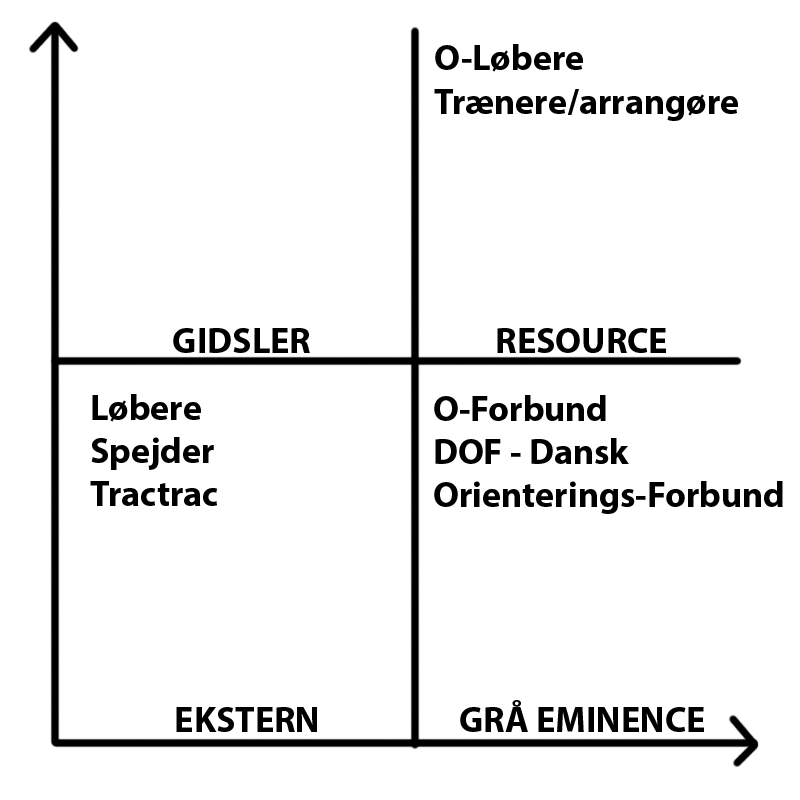
\includegraphics[width=0.70\textwidth]{billeder/Medvirken-indflydelse}
\vspace{0.25cm}

HUSK AT LAVE BILLEDET OM!!



\subsection{Opsummering}
Ud fra interessentanalysen, er gruppen kommet frem til at o-løberne og trænerne, er de vigtigste interessenter, og er derfor også blevet sat som ressourcepersoner i dette projekt. Derfor har gruppen valgt at kontakte de to grupper af interessenter, og gennemføre et interview med dem. 

